%%%%%%%%%%%%%%%%%%%%%%%%%%%%%%%%%%%%%%%%%%%%%%%%%%%%%%%%%%%%%%%%%%%%%
% 																    %
% 	Class pgffigure for easier plots using pgfplots					%
%																	%
%	Possible options:												%
%   nofinal|final - draws 1cm grid on background or 				%
%                   disables grid. final by default.				%
%   nocyr|cyr - usage western or cyrillic numbers notation:			%
%               cyr enables comma `,' instead of dot `.' and		%
%               removes dot as thouthands separator.				%
%               nocyr by default.									%
%																	%
%																	%
%%%%%%%%%%%%%%%%%%%%%%%%%%%%%%%%%%%%%%%%%%%%%%%%%%%%%%%%%%%%%%%%%%%%%

\documentclass[final]{pgffigure}
\usepackage[utf8]{inputenc}
\usepackage{mathrsfs}
\usepackage{xcolor}

\pagestyle{empty}

\renewcommand{\vec}[1]{\bm{#1}}

\usetikzlibrary{patterns,fit}
\usepgfplotslibrary{fillbetween}

% colors definition
\definecolor{colj0}{HTML}{D73240}
\definecolor{colj1}{HTML}{00E745}
\definecolor{colj2}{HTML}{A600F2}
\definecolor{colj3}{HTML}{FC9A0E}
\definecolor{colj4}{HTML}{0000F2}

\begin{document}
	
	\begin{tikzpicture}[helpgrid]
		\Large
		% text on stripe
		\node at (0,0) {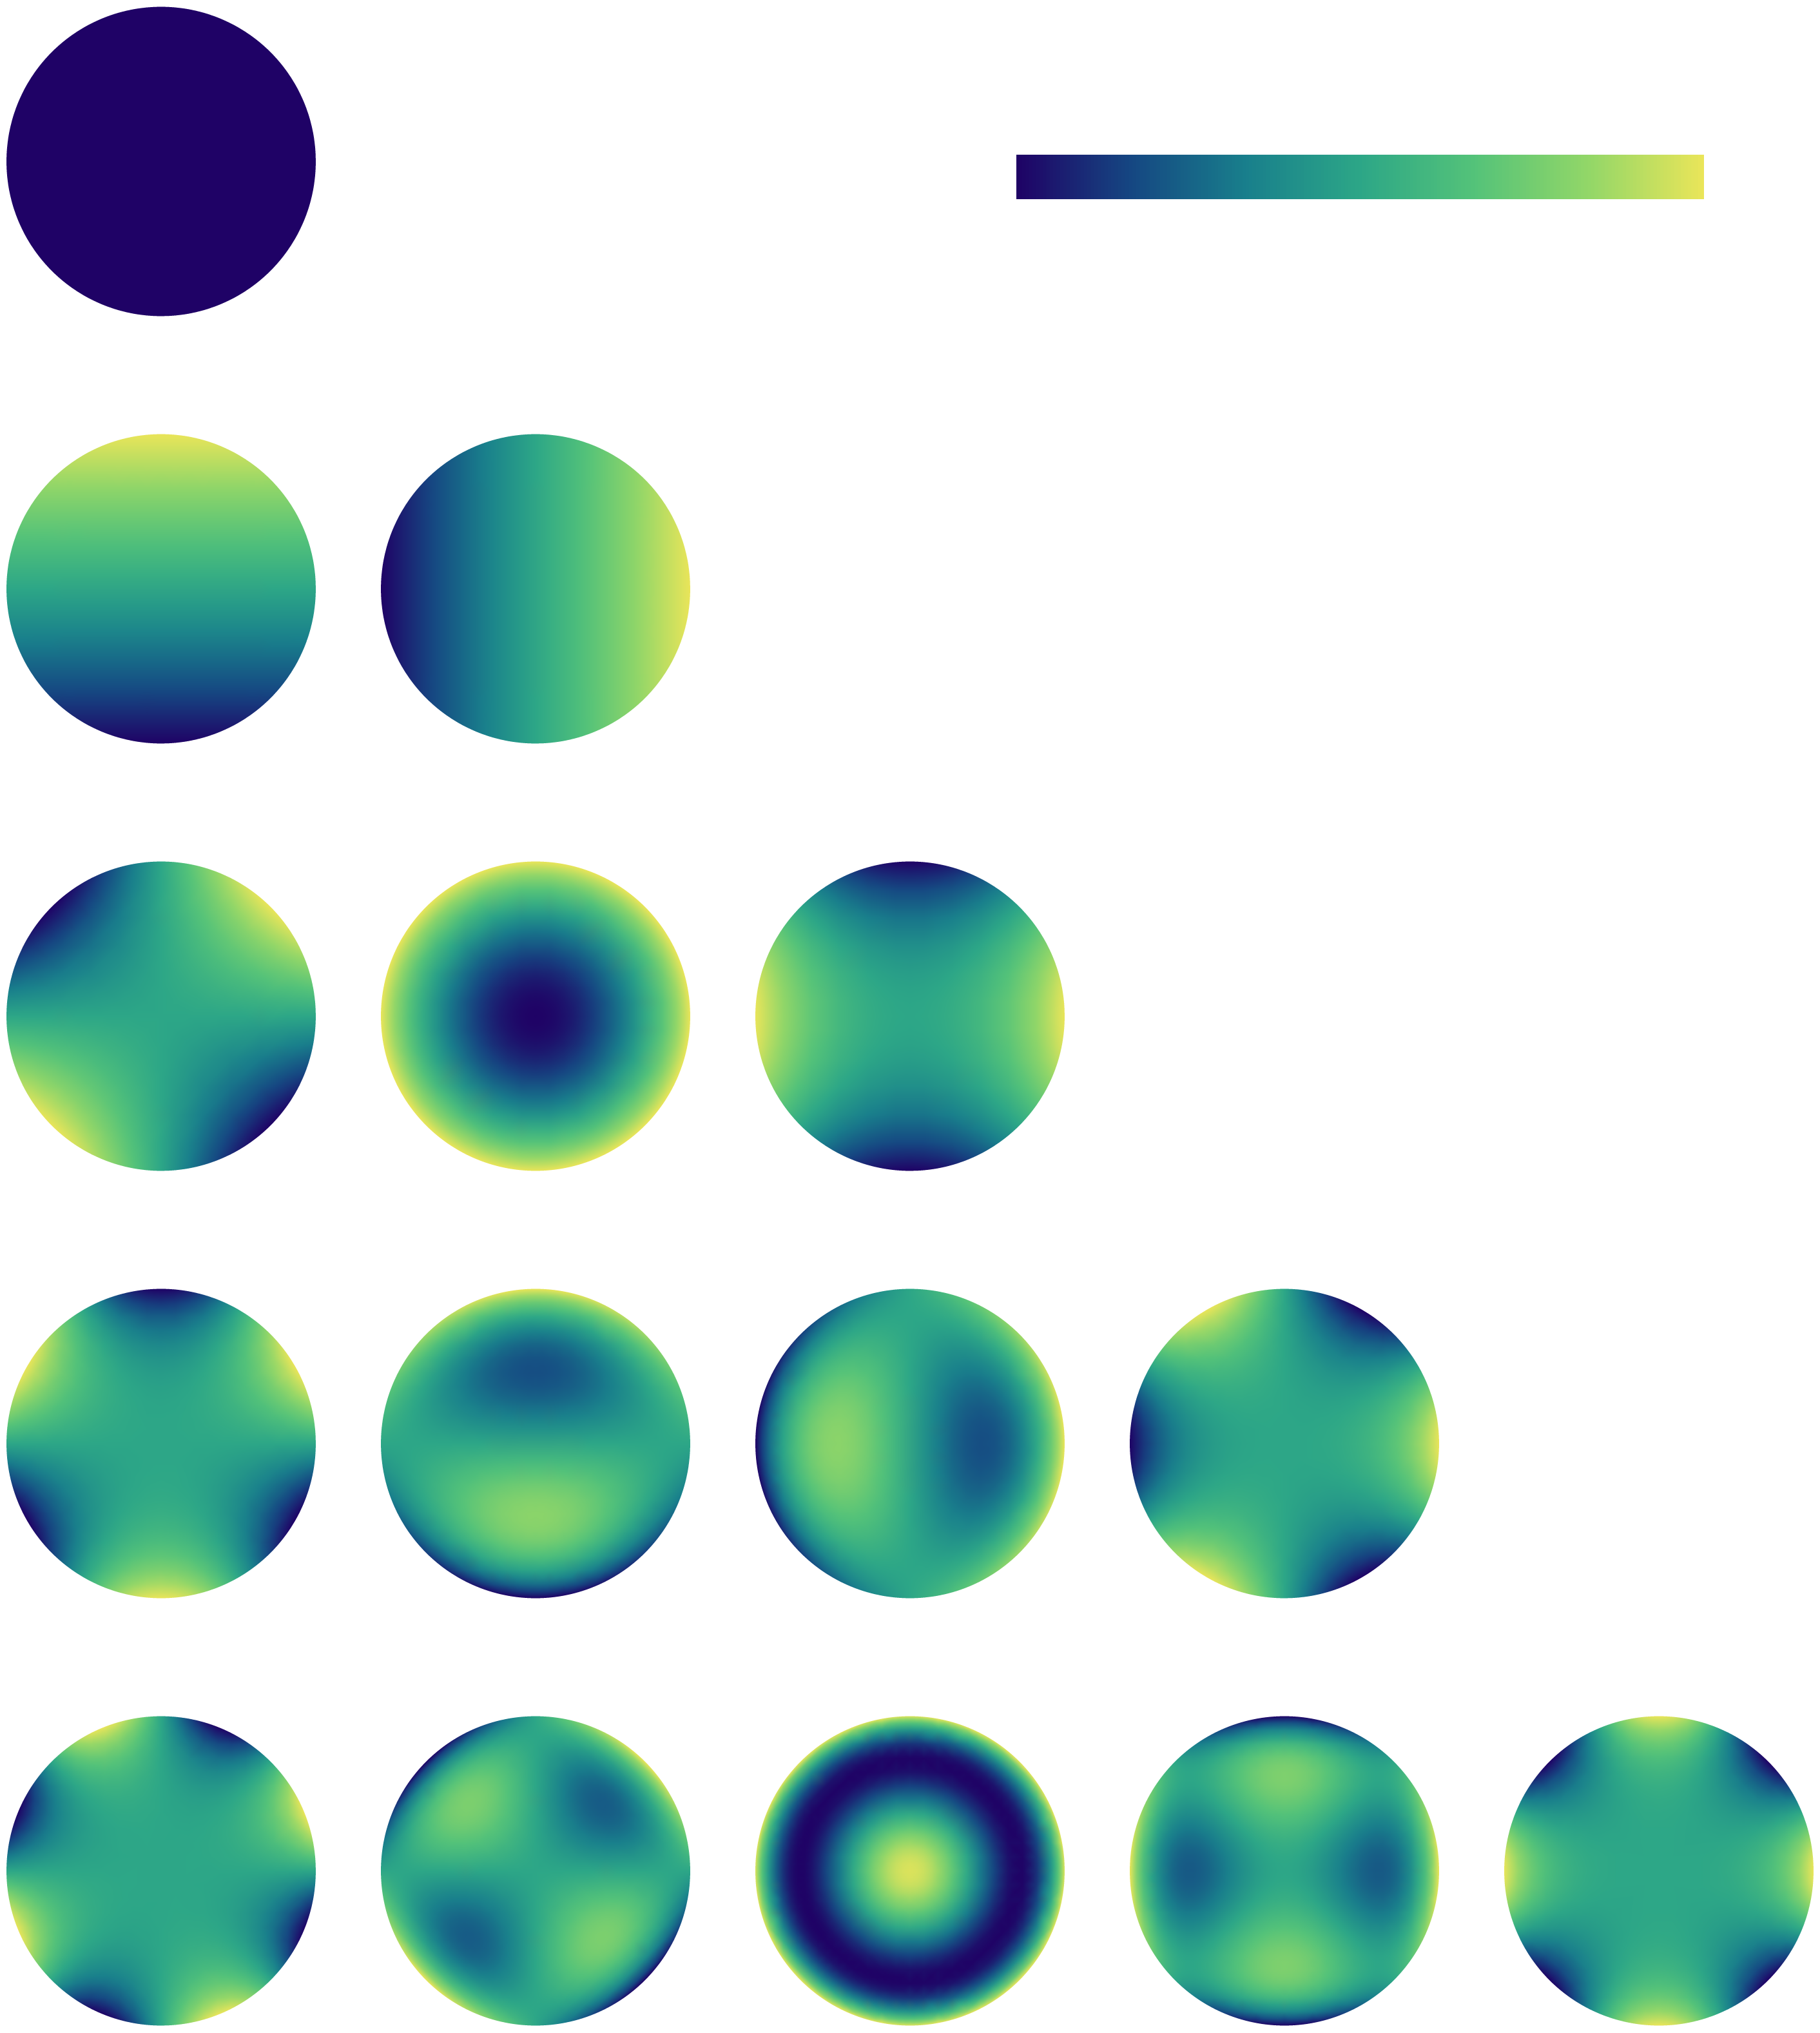
\includegraphics[width=\textwidth]{modes2d.png}};
		% legend 
		\node at (1.1, 6) { $\text{min}$ };
		\node at (4.8, 6) { $\text{max}$ };
		% n
		\node at (-6.8, 5.5) { $n = 0$ };
		\node at (-6.8, 3.1) { $n = 1$ };
		\node at (-6.8, 0) { $n = 2$ };
		\node at (-6.8, -2.9) { $n = 3$ };
		\node at (-6.8, -5.8) { $n = 4$ };
		% l 
		% n = 0
		\node at (-5, 4.4) { $l = 0$ };
		% n = 1
		\node at (-5, 1.5) { $l = -1$ };
		\node at (-2.4, 1.5) { $l = 1$ };
		% n = 2
		\node at (-5, -1.3) { $l = -2$ };
		\node at (-2.4, -1.3) { $l = 0$ };
		\node at (0, -1.3) { $l = 2$ };
		% n = 3
		\node at (-5, -4.1) { $l = -3$ };
		\node at (-2.4, -4.1) { $l = -1$ };
		\node at (0, -4.1) { $l = 1$ };
		\node at (2.5, -4.1) { $l = 3$ };
		% n = 4
		\node at (-5, -7) { $l = -4$ };
		\node at (-2.4, -7) { $l = -2$ };
		\node at (0, -7) { $l = 0$ };
		\node at (2.5, -7) { $l = 2$ };
		\node at (5, -7) { $l = 4$ };
	\end{tikzpicture}
	
\end{document}

